\documentclass[a4j]{jarticle}
\renewcommand{\baselinestretch}{0.85}
\usepackage[top=1.5cm, bottom=1.5cm, left=1.5cm, right=1.5cm]{geometry}
\usepackage[dvipdfmx]{graphicx}
\usepackage{subfig}
\usepackage{float}

\begin{document}

	\begin{flushright}
		MDLabグループミーティング資料\\
		25年6月3日(火)
	\end{flushright}

	\begin{center}
		{\Large	疑似ラベルを用いた自動運転のための遠赤外線画像からの物体検出}
	\end{center}

	\begin{flushright}
		{\large B4 加藤 達也}
	\end{flushright}

	\section{研究背景および目的}
	\begin{itemize}
		\item 背景: 完全自動運転の実用化に向けて技術の開発が進められており、その為に車載カメラ画像からの物体検出は重要な要素技術である。可視光画像からの物体検出は天候や時間帯によって精度が低下するので、その解決策として遠赤外線からの物体検出手法を考える。
		\item 課題:遠赤外線画像のデータセットは可視光画像のデータセットと比較して数が少ない。
		\item 目的: 遠赤外線画像を入力として低照度下でも安定的に動作する検出モデルを構築する。また、RGB画像に適応して得た検出領域を教師とするドメイン適応を用いて、遠赤外線領域における検出モデルを構築する。
	\end{itemize}
	\begin{figure}[ht]
		%複数の図を並べて出力する方法%
		\centering
		\begin{minipage}[b]{0.3\columnwidth}
			\centering
			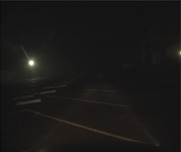
\includegraphics[height=3cm]{fig/RGB.png}%
			\caption{RGB画像}
		\end{minipage}
		\begin{minipage}[b]{0.3\columnwidth}
			\centering
			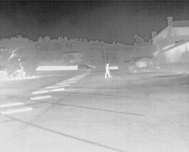
\includegraphics[height=3cm]{fig/FIR.png}%
			\caption{FIR画像}
		\end{minipage}
		\begin{minipage}[b]{0.35\columnwidth}
			\centering
			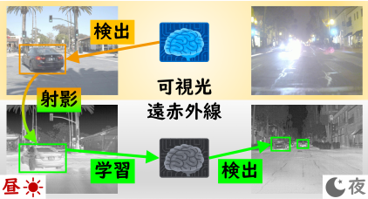
\includegraphics[height=3cm]{fig/domain_adaptation.png}%
			\caption{ドメイン適応の流れ}
		\end{minipage}
	\end{figure}
	\section{これまでの研究のまとめ}
	\begin{itemize}
		\item 谷本先輩の最終的な提案手法は以下の通りである。流れとしては図4(a)の通りである。
		\begin{enumerate}
			\item RGB画像に対して高精度な可視光モデルを用いて物体検出を行い、その結果をFIR画像に変換して疑似ラベルを生成する。
			\item 可視光モデルの出力信頼度に基づき、高信頼の検出結果のみを疑似ラベルとして使用し、誤学習を防止する。
			\item FIR画像と疑似ラベルを用いて、可視光モデルをファインチューニングし、FIR画像専用の物体検出モデルを構築する。
		\end{enumerate}
	\end{itemize}
	\begin{figure}[H]
		\centering%
		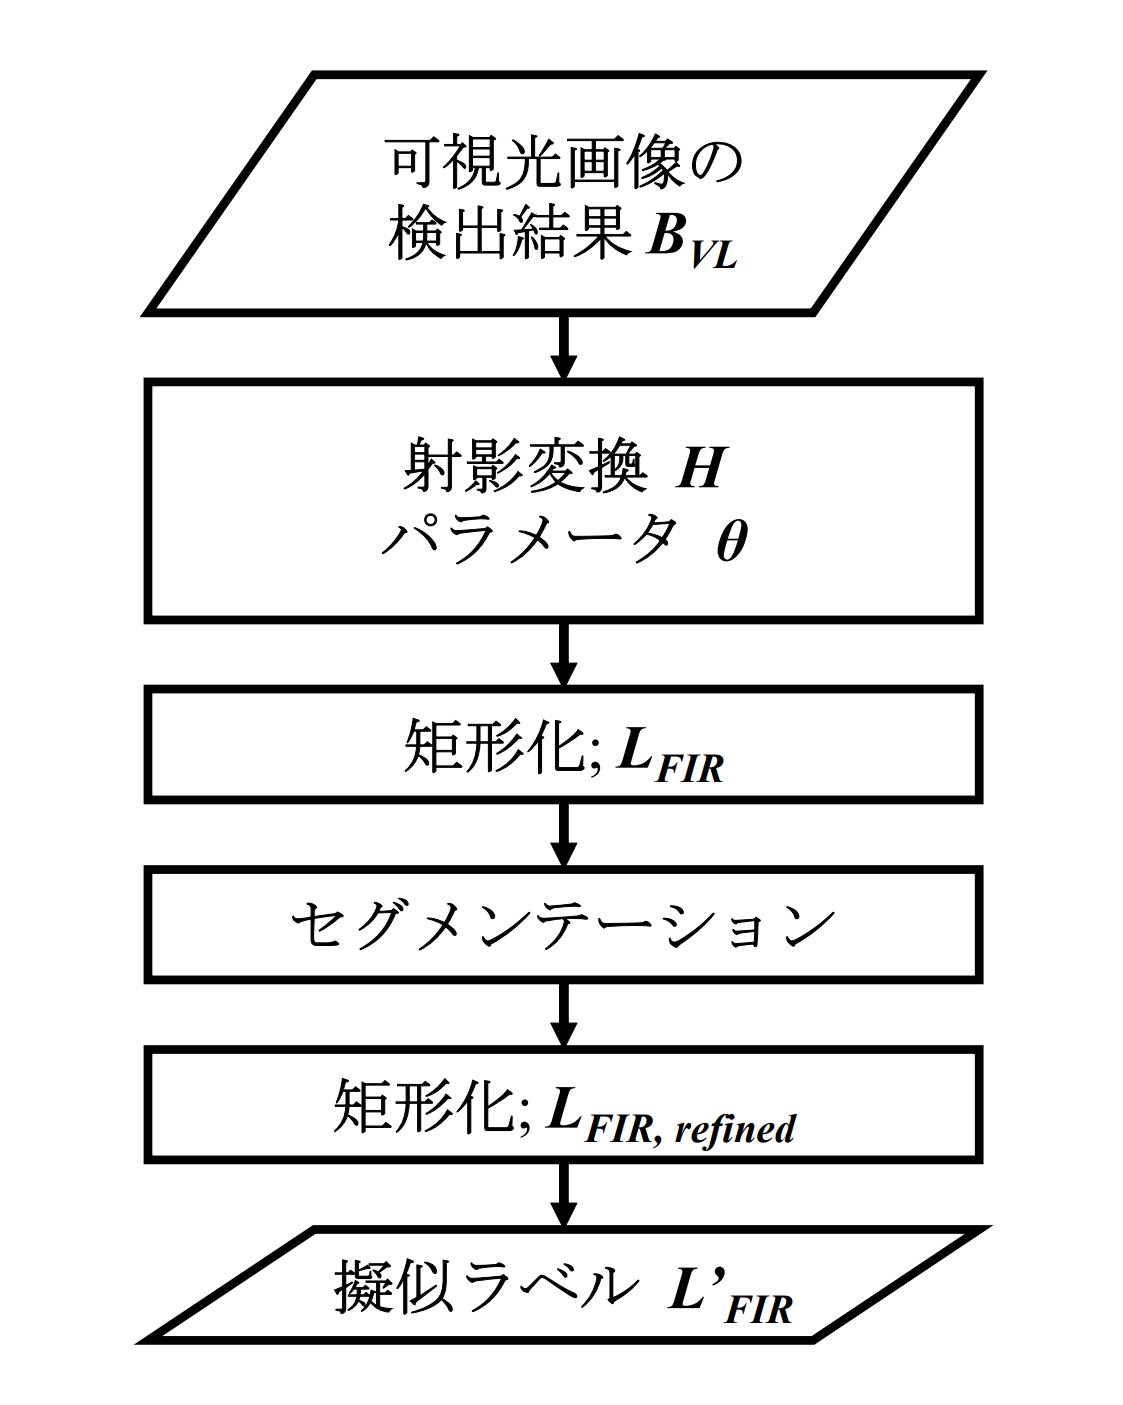
\includegraphics[height=6cm]{fig/疑似ラベル生成の流れ.png}
		\hspace{1cm}%
		\caption{疑似ラベル作成までの流れ}
		\label{fig:Research summary}%
	\end{figure}
	\begin{itemize}
		\item 損失関数のカスタマイズを行った。採用した損失関数はFocalLossとL1Loss。
		\item クラス分類とオブジェクト性にFocalLoss、バウンディングボックス回帰にSmoothL1Lossを使用した。
		\item 現在、サイズが小さいオブジェクトに対しての精度が低いため、難しいサンプルに着目し、分類性能を向上させるFocalLossを採用した。
		\item SmoothL1Lossに関してはYOLOXで中心座標と幅、高さの回帰に対してL1距離を使うことが多いため、採用した。
	\end{itemize}
	\begin{table}[htbp]
		\centering
		\begin{tabular}{|c|c|c|c|c|c|c|}
			\hline
			\textbf{Category} & \textbf{mAP} & \textbf{mAP\_50} & \textbf{mAP\_75} & \textbf{mAP\_s} & \textbf{mAP\_m} & \textbf{mAP\_l} \\
			\hline
			person & 0.039 & 0.194 & 0.001 & 0.039 & 0.079 & 0.087 \\
			car    & 0.163 & 0.490 & 0.055 & 0.039 & 0.322 & 0.644 \\
			\hline
		\end{tabular}
		\caption{各カテゴリの検出精度(mAP)}
	\end{table}
	\section{前回のGMからの進捗}
	\subsection{損失関数の実装について}
	\begin{itemize}
		\item configファイルはbaseファイルに上書きや追加をすることによってカスタマイズをする構造になっているが、改めてbaseファイルの方を参照して見たところ、既に損失関数は実装されていた。
		\item bboxにはIoULoss、クラス分類とオブジェクト性にCrossEntropyLossが使用されていた。
		\item この2つとも、Yoloxに最初から実装されている損失関数であったため、デフォルトの損失関数から他のカスタマイズされた損失関数に変更することによってどのように検出精度が向上するかを考えるべきであると思った。
	\end{itemize}
	\subsection{アノテーションファイルの改善検討}
	\begin{table}[htbp]
		\centering
		\begin{tabular}{|l|l|}
			\hline
			\textbf{項目} & \textbf{値} \\
			\hline
			base\_lr & $1.0000 \times 10^{-2}$ \\
			lr & $1.0000 \times 10^{-2}$ \\
			eta & 2:10:43 \\
			time & 0.2130 \\
			data\_time & 0.0158 \\
			memory & 11174 \\
			loss & 0.0021 \\
			loss\_cls & 0.0000 \\
			loss\_bbox & 0.0021 \\
			loss\_obj & 0.0000 \\
			\hline
		\end{tabular}
		\caption{mmengine の学習ログ(Epoch 169, iteration 250)}
	\end{table}
	\begin{itemize}
		\item 表2のloss\_cls、loss\_objの値が0となっている。
		\item 原因不明なので、損失関数のパラメータを変更して変化するかを確かめたい。
	\end{itemize}
	\subsection{クラス数の訂正}
	\begin{itemize}
		\item いままでコード内でクラス数が80と記述されていた部分があったが、2に統一したところ、検出精度の改善が見られた。(実験の最初の部分のみの切り取り)
	\end{itemize}
	\begin{table}[ht]
		\centering
		\caption{各クラスにおける性能比較(旧モデル vs 新モデル)}
		\begin{tabular}{llll}
			\hline
			クラス & 指標 & 以前(旧) & 今回(新) \\
			\hline
			\textbf{person} & mAP      & 0.034 & 0.017 \\
							& mAP\_50  & 0.126 & 0.063 \\
			\textbf{car}    & mAP      & 0.000 & 0.066 \\
							& mAP\_50  & 0.000 & 0.221 \\
			\hline
		\end{tabular}
	\end{table}
	\subsection{ITSミーティングについて}
	\begin{itemize}
		\item 愛知工科大学の久徳先生との毎週月曜日に行われるITSミーティングにおいて、アドバイスをいただいた。
		\item クラス数が80であった部分は学習時点では80で、最後のファインチューニング時にクラス数を2に絞ることを意図として谷本先輩が設定していた。
		\item 損失関数については既存の損失関数はそれぞれ想定された使い方が存在するので、それに従って適した損失関数を各所に実装する。
		\item 既存の損失関数でも良いが、谷本先輩は独自の計算での損失関数の作成を目指していた。
	\end{itemize}
	\section{今後の課題\&スケジュール}
		\begin{itemize}
			\item FLIRのバージョンアップをする。
			\item 損失関数に関する理解を深め、より良い検出精度を目指す。できれば独自の計算で損失関数を作成したい。
		\end{itemize}
\end{document}
